{\color{gray}\hrule}
\begin{center}
\section{Methodology}
\bigskip
\end{center}
{\color{gray}\hrule}
\subsection{Data Preparation}

As mentioned earlier, the \textit{Song of Ice and Fire} series was widely available online in the ".pdf" format; thus, these books were gathered in that format for this project. Then using the python library, PyPDF2, we converted them to ".txt" files, and cleaned them. Since the OpenAI model has a token limit and the RAG/KRAG architecture includes the most relevant files in the context of the prompt, the text files were split up in chunks of a thousand characters to reduce the amount of tokens in the prompt when retrieving files or in this case retrieving "chunks".

\subsection{Named Entity Recognition (NER)}

For the named entity recognition portion of the project, there were issues building the model from scratch; so, in order to make progress in a timely manner, spaCy's English "en\_core\_web\_sm" model was used in addition to the "sentencizer" pipe to split up sentences from a sequence. For each chunk of text, the NER model split up the sentences using aforementioned sentencizer and tokenized each sentence for entities, subjects, grammatical objects, and root relationship between the two returning them attributes in a "Doc" object.

\subsection{Relationship Extraction/Knowledge Graph Construction}

The knowledge graph was constructed using the NER model's returned "Doc" object. Entities were retrieved from this "Doc" object and relationships between entities for each sentence in given chunks were parsed for subject, grammatical object, and root relationship between the two. Entities and relationships were passed to the networkx module to construct a knowledge graph for given chunks.
\par
As a quick example, take the sentences "Mary reads a book. Nancy eats pickles." Treating this string as a "chunk" passed to the NER model, it recognizes the entities "Mary" and "Nancy" and stores them in the "ent" attribute in a "Doc" object. The model splits the sentences into two, stores them in its Doc's "sents" attribute, and for each sentence stores the sentence's grammatical subject, object, and root relationship between the two. In this example, "Doc.sents" is an attribute of a generator object containing the two sentences: \bigskip

\begin{center}
["Mary reads a book.", "Nancy eats pickles"]
\end{center}
\bigskip

For the first sentence, "Mary" is stored as the subject, "book" is stored as the grammatical object, and "reads" is stored as the the root relationship between the subject and object. After these entities are recognized, sentences are split, and relationships are recognized, passing these variables to the networkx module and visualizing the graph using matplotlib.pyplot gives the following result. Noticeably the direction of the arrow goes from grammatical subject to object and the edges between nodes do not visibly have the root relationships, but they are implied.

\begin{figure}[h]
    \centering
    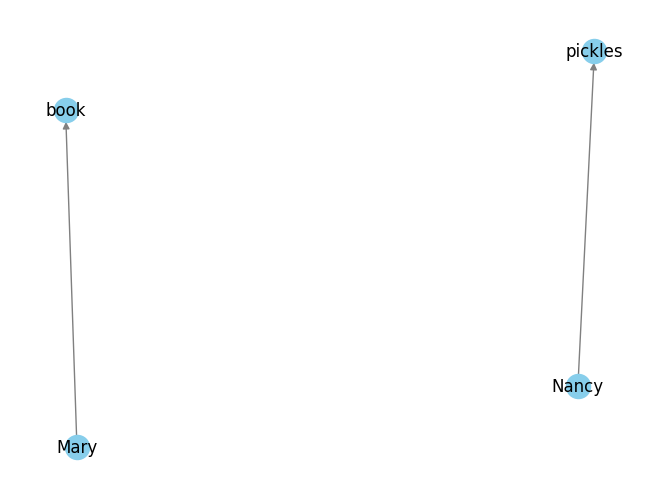
\includegraphics[width=0.75\linewidth]{images/example_kg.png}
    \caption{Knowledge Graph for Example Chunk}
    \label{fig:enter-label}
\end{figure}

\newpage

Repeating the same process for the first fifteen chunks of \textit{"A Game of Thrones"} results in the following graph.

\begin{figure}[h]
    \centering
    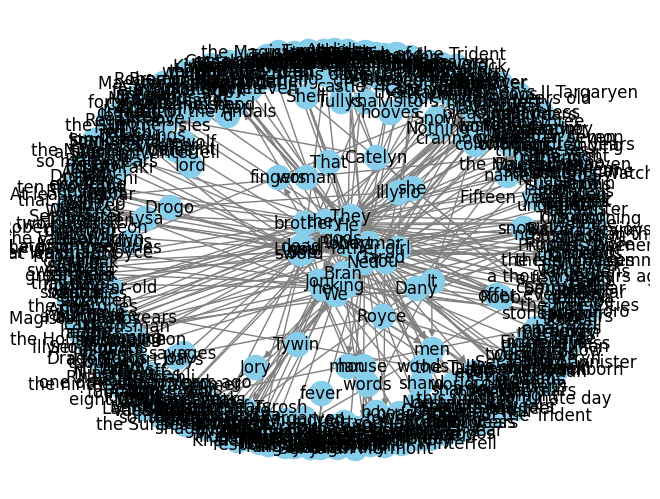
\includegraphics[width=0.75\linewidth]{images/15_chunk_got_kg.png}
    \caption{Knowledge Graph for First Fifteen Chunks of \textit{A Game of Thrones}}
    \label{fig:enter-label}
\end{figure} \par

This process was repeated to generate a knowledge graph for all chunks containing two given books in the series.

\bigskip